\section{Частица в однородном силовом поле}

Пусть сила, действующая на частицу, равна $F$ по модулю и направлена вдоль оси $z$ в обратном направлении. Гамильтониан в классическом случае:
\[
	\hat{H} = \frac{\hat{p}_z^2}{2m} + F \hat{z} 
\]
Уравнение Шрёдингера:
\[
	\frac{p_z^2}{2m} C(p_z, t) + i \hbar F \frac{\partial C(p_z, t)}{\partial p_z} = i\hbar \frac{\partial C(p_z, t)}{\partial t}
\]
Вместо $\lambda$ будет выступать $-iE/\hbar$. Для $Y$ получаем уравнение
\[
	\frac{p_z^2}{2m} Y + i \hbar F \frac{\partial Y}{\partial p_z} = E Y
\]
Будем искать $Y$ в форме $\exp f(p_z)$:
\[
	i \hbar F \frac{\partial f(p_z)}{\partial p_z} = E - \frac{p_z^2}{2m}
\]
\[
	f(p_z) = - i \frac{E}{\hbar F} p_z + i \frac{1}{6 m \hbar F} p_z^3 + const
\]
Константа уйдёт в нормировочный множитель. 
\[
	Y(p_z, E) = A \exp \left(-\frac{i}{\hbar} \left( \frac{E}{F} p_z - \frac{1}{6 m F} p_z^3 \right) \right)
\]
\[
	Y^{-1}(p_z, E) = B \exp \left(\frac{i}{\hbar} \left( \frac{E}{F} p_z - \frac{1}{6 m F} p_z^3 \right) \right)
\]
\[
	AB \int\limits_{-\infty}^{\infty} \exp \left(\frac{i p_z}{\hbar F} (E' - E) \right) dp_z = 
	2\pi AB\hbar F\, \delta(E' - E) = \delta(E' - E)
\]
Откуда можно в качестве $A$ и $B$ можно взять константы:
\[
	A = B = \frac{1}{\sqrt{2\pi \hbar F}}
\]
\[
	\begin{gathered}
		C(p_z, t) = \int\limits_{-\infty}^{\infty} C(p_z, 0) \int\limits_{-\infty}^{\infty} AB
		\exp \left(-\frac{i}{\hbar} \left( E \left(\frac{p_z - p_z'}{F} + t\right) - \frac{1}{6 m F} (p_z^3 - p_z'^3) \right)
		\right)\, dE\, dp_z' = \\
		=
		\int\limits_{-\infty}^{\infty} C(p_z', 0) \delta(p_z - p_z' + F t) 
		\exp \left(\frac{i}{6 m \hbar F} (p_z^3 - p_z'^3) \right)
		\, dp_z' = \\
		=
		C(p_z + F t, 0) \exp \left(\frac{i(-3 p_z^2 F t - 3 p_z F^2 t^2 - F^3 t^3)}{6 m \hbar F} \right) = \\
		=
		C(p_z + F t, 0) \exp \left(-\frac{i}{\hbar} \left(\frac{p_z^2}{2m} t + \frac{p_z F t^2}{2 m} + \frac{F^2 t^3}{6 m}\right) \right)
	\end{gathered}
\]
Чтобы получить дискретный спектр нужно ввести дополнительные условия. Чаще всего таким условием выступает поверхность, за пределы которой частица не может попасть. В качестве такой поверхности может выступать поверхность Земли для поля тяжести, обкладка конденсатора.

\section{Гауссовский волновой пакет в однородном поле}

Пусть
\[
	\psi(z, 0) = \frac{1}{\sqrt[4]{2\pi \sigma^2}} \exp \left( -\frac{(z - z_0)^2}{4\sigma^2}\right)
\]
\[
	\begin{gathered}
		C(p_z, 0) = \frac{1}{\sqrt[4]{2\pi \sigma^2}}\frac{1}{(2\pi\hbar)^{1/2}} \int\limits_{-\infty}^{\infty} \exp \left(-\frac{(z - z_0)^2}{4\sigma^2} - \frac{i}{\hbar} p_z z  \right) dz = \\
		=
		\frac{1}{\sqrt[4]{2\pi \sigma^2}}\frac{1}{(2\pi\hbar)^{1/2}} \exp\left(-\frac{i}{\hbar}p_z z_0\right)\int\limits_{-\infty}^{\infty} \exp \left(-\frac{(z - z_0)^2}{4\sigma^2} - \frac{i}{\hbar} p_z (z - z_0)  \right) dz = \\
		=
		\frac{1}{\sqrt[4]{2\pi \sigma^2}}\frac{1}{(2\pi\hbar)^{1/2}} \exp\left(-\frac{i}{\hbar}p_z z_0\right)
		\int\limits_{-\infty}^{\infty} \exp \left(-\frac{(z - z_0)^2}{4\sigma^2} - 2 \frac{i}{\hbar} \sigma p_z \frac{(z - z_0)}{2 \sigma}  \right) dz = \\
		=
		\frac{1}{\sqrt[4]{2\pi \sigma^2}}\frac{1}{(2\pi\hbar)^{1/2}} \exp\left(-\frac{i}{\hbar}p_z z_0\right)
		\int\limits_{-\infty}^{\infty} \exp \left(-\left(\frac{(z - z_0)}{2 \sigma} + \frac{i}{\hbar} \sigma p_z \right)^2 - \frac{\sigma^2 p_z^2}{\hbar^2}  \right) dz = \\
		=
		\frac{2\sqrt[4]{2\pi \sigma^2}}{(2\pi\hbar)^{1/2}} \exp\left(-\frac{i}{\hbar}p_z z_0 - \frac{\sigma^2 p_z^2}{\hbar^2} \right) = \\
		=
		\sqrt[4]{\frac{2\sigma^2}{\pi \hbar^2}} \exp\left(-\frac{i}{\hbar}p_z z_0 - \frac{\sigma^2 p_z^2}{\hbar^2} \right)
	\end{gathered}
\]
\[
	\begin{gathered}
		\langle z \rangle =
		\sqrt{\frac{2\sigma^2}{\pi \hbar^2}} 
		\int\limits_{-\infty}^{\infty} \left(z_0 - \frac{2i\hbar \sigma^2}{\hbar^2} (p_z + Ft) + \frac{p_z}{m} t +  \frac{F t^2}{2m}\right) 
		\exp\left( - \frac{2\sigma^2 (p_z + Ft)^2}{\hbar^2} \right) dp_z = \\
		=
		\sqrt{\frac{2\sigma^2}{\pi \hbar^2}} 
		\int\limits_{-\infty}^{\infty} \left(z_0 - \frac{2i\hbar \sigma^2}{\hbar^2} (p_z + Ft) + \frac{p_z + F t}{m} t -  \frac{F t^2}{2m}\right) 
		\exp\left( - \frac{2\sigma^2 (p_z + Ft)^2}{\hbar^2} \right) dp_z = \\
		=
		z_0 - \frac{F t^2}{2m}	
	\end{gathered}
\]
\[
	\begin{gathered}
		\langle z^2 \rangle =
		\sqrt{\frac{2\sigma^2}{\pi \hbar^2}} 
		\int\limits_{-\infty}^{\infty} \left(z_0 - \frac{F t^2}{2m} + \left(\frac{t}{m}- 2\frac{i \sigma^2}{\hbar}\right) (p_z + Ft)\right)^2
		\exp\left( - \frac{2\sigma^2 (p_z + Ft)^2}{\hbar^2} \right) dp_z + \\
		+
		\sqrt{\frac{2\sigma^2}{\pi \hbar^2}} 
		\int\limits_{-\infty}^{\infty} \left(2\sigma^2 + \frac{i\hbar}{m} t \right)
		\exp\left( - \frac{2\sigma^2 (p_z + Ft)^2}{\hbar^2} \right) dp_z = \\
		=
		\left(z_0 - \frac{F t^2}{2m}\right)^2 +
		\left(\frac{t}{m}- 
		2\frac{i \sigma^2}{\hbar}\right)^2 \frac{\hbar^2}{4 \sigma^2} +
		\left(2\sigma^2 + \frac{i\hbar}{m} t \right) = \\
		=
		\left(z_0 - \frac{F t^2}{2m}\right)^2 +
		\frac{t^2\hbar^2}{4 m^2 \sigma^2} + \sigma^2
	\end{gathered}
\]
Дисперсия:
\[
	\langle z^2 \rangle - \langle z \rangle^2 =
	\frac{t^2\hbar^2}{4 m^2 \sigma^2} + \sigma^2
\]

\section{Частица в однородном поле над непроницаемым барьером}

Рассмотрим частицу в треугольной потенциальной яме:

\parbox{\textwidth}{
	\centering
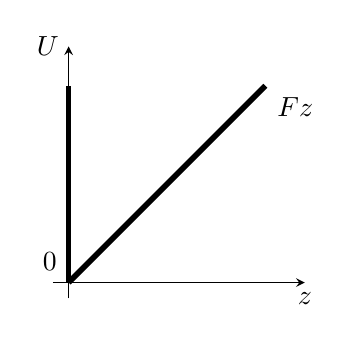
\begin{tikzpicture}[>= stealth]
\draw[->] (0, -0.2) -- (0, 3) node[left]{$U$};
\draw[->] (-0.2, 0) -- (3, 0) node[below]{$z$};
\draw[line width = 2pt] (0, 0) node[above left]{$0$} -- (0, 2.5);
\draw[line width = 2pt] (0, 0) -- (2.5, 2.5) node[below right]{$F z$}; 
\end{tikzpicture}
}
В этом случае спектр дискретный. Нам необходимо от импульсной формы перейти к координатной. В этом случае получится обычное стационарное уравнение Шрёдингера c решением:
\[
	\begin{gathered}
	\psi(z, E) = \int\limits_{-\infty}^{\infty} 
	A \exp \left(-\frac{i}{\hbar} \left( \frac{E - Fz}{F} p_z - \frac{1}{6 m F} p_z^3 \right) \right) dp_z = \\ =
	\int\limits_{-\infty}^{\infty} 
	A \cos \left( -\frac{E - Fz}{F \hbar} p_z + \frac{1}{2 m F \hbar} \frac{p_z^3}{3} \right) dp_z
	= \\ =
	A (2 m F \hbar)^{1/3} \mathrm{\,Ai\,} \left((2 m F \hbar)^{1/3}\frac{Fz - E}{F \hbar}\right)	
	\end{gathered}
\]
Зная корни функции Эйри $x_1, x_2, \ldots$, легко найти спектр:
\[
	E_k = - (2 m)^{-1/3} \hbar^{2/3} F^{2/3} x_k
\]
А воспользовавшись интегралом:
\[
	\int\limits_{x_k}^{\infty} \mathrm{\,Ai\,}^2 (x)\,dx = \left[\mathrm{\,Ai\,}' (x_k)\right]^2,
\]
нормировочную константу:
\[
	A = \hbar^{-2/3} (2 m F)^{-1/6} |\mathrm{\,Ai\,}' (x_k)|^{-1}
\]
Окончательно волновые функции:
\[
	\psi_k(z) = \frac{(2mF)^{1/6}}{\hbar^{1/3}|\mathrm{\,Ai\,}' (x_k)|} \mathrm{\,Ai\,} \left((2 m F \hbar)^{1/3} \frac{z}{\hbar} + x_k \right)
\]
Для электронов:
\[
	E_k \approx -1{,}14\times10^{6} F^{2/3} x_k \text{ эВ}
\]
Найдём количество значений $x_k$ приходящихся на интервал $(k_{b}T, k_{b}(T + \Delta T))$ при $\Delta T= 10 $К и $T = 300 $К (обозначим эту величину $N$) для поля силы тяжести, что соответствует частице над поверхностью Земли. Для этого воспользуемся приближённым выражением:
\[
	\mathrm{Ai\,}(x) \underset{x \to -\infty}{\approx} \frac{1}{\sqrt{\pi} x^{1/4}} \sin \left( \frac{2}{3} |x|^{3/2} + \frac{\pi}{4}\right)
\]
\[
	|x_k|^{3/2} \approx \frac{3}{2}\pi k - \frac{3\pi}{8}
\]
\[
	N \approx \frac{2^{3/2}}{3\pi g \hbar m^{1/2}} k_{b}^{3/2} T^{3/2} ((1 + \Delta T/T)^{3/2} - 1) \approx 
	\frac{2^{1/2}}{\pi g \hbar m^{1/2}} k_{b}^{3/2} T^{1/2} \Delta T
\]
Для электронов:
\[
	N \approx 4{,}07\times10^{15}
\]
Далее можно приближённо вычислить среднюю температуру таких частиц и так далее.